\documentclass{article}

\usepackage{graphicx}
\usepackage{tikz}
\usepackage{tikzsymbols}
\usetikzlibrary{calc,patterns,shapes.geometric}
\pagestyle{empty}
\usepackage[margin=0pt]{geometry}
\geometry{papersize={14in,12in}}

\def\centerarc[#1](#2)(#3:#4:#5){\draw[#1] ($(#2)+({#5*cos(#3)},{#5*sin(#3)})$) arc (#3:#4:#5);}

\begin{document}
	\begin{figure}
		\centering
		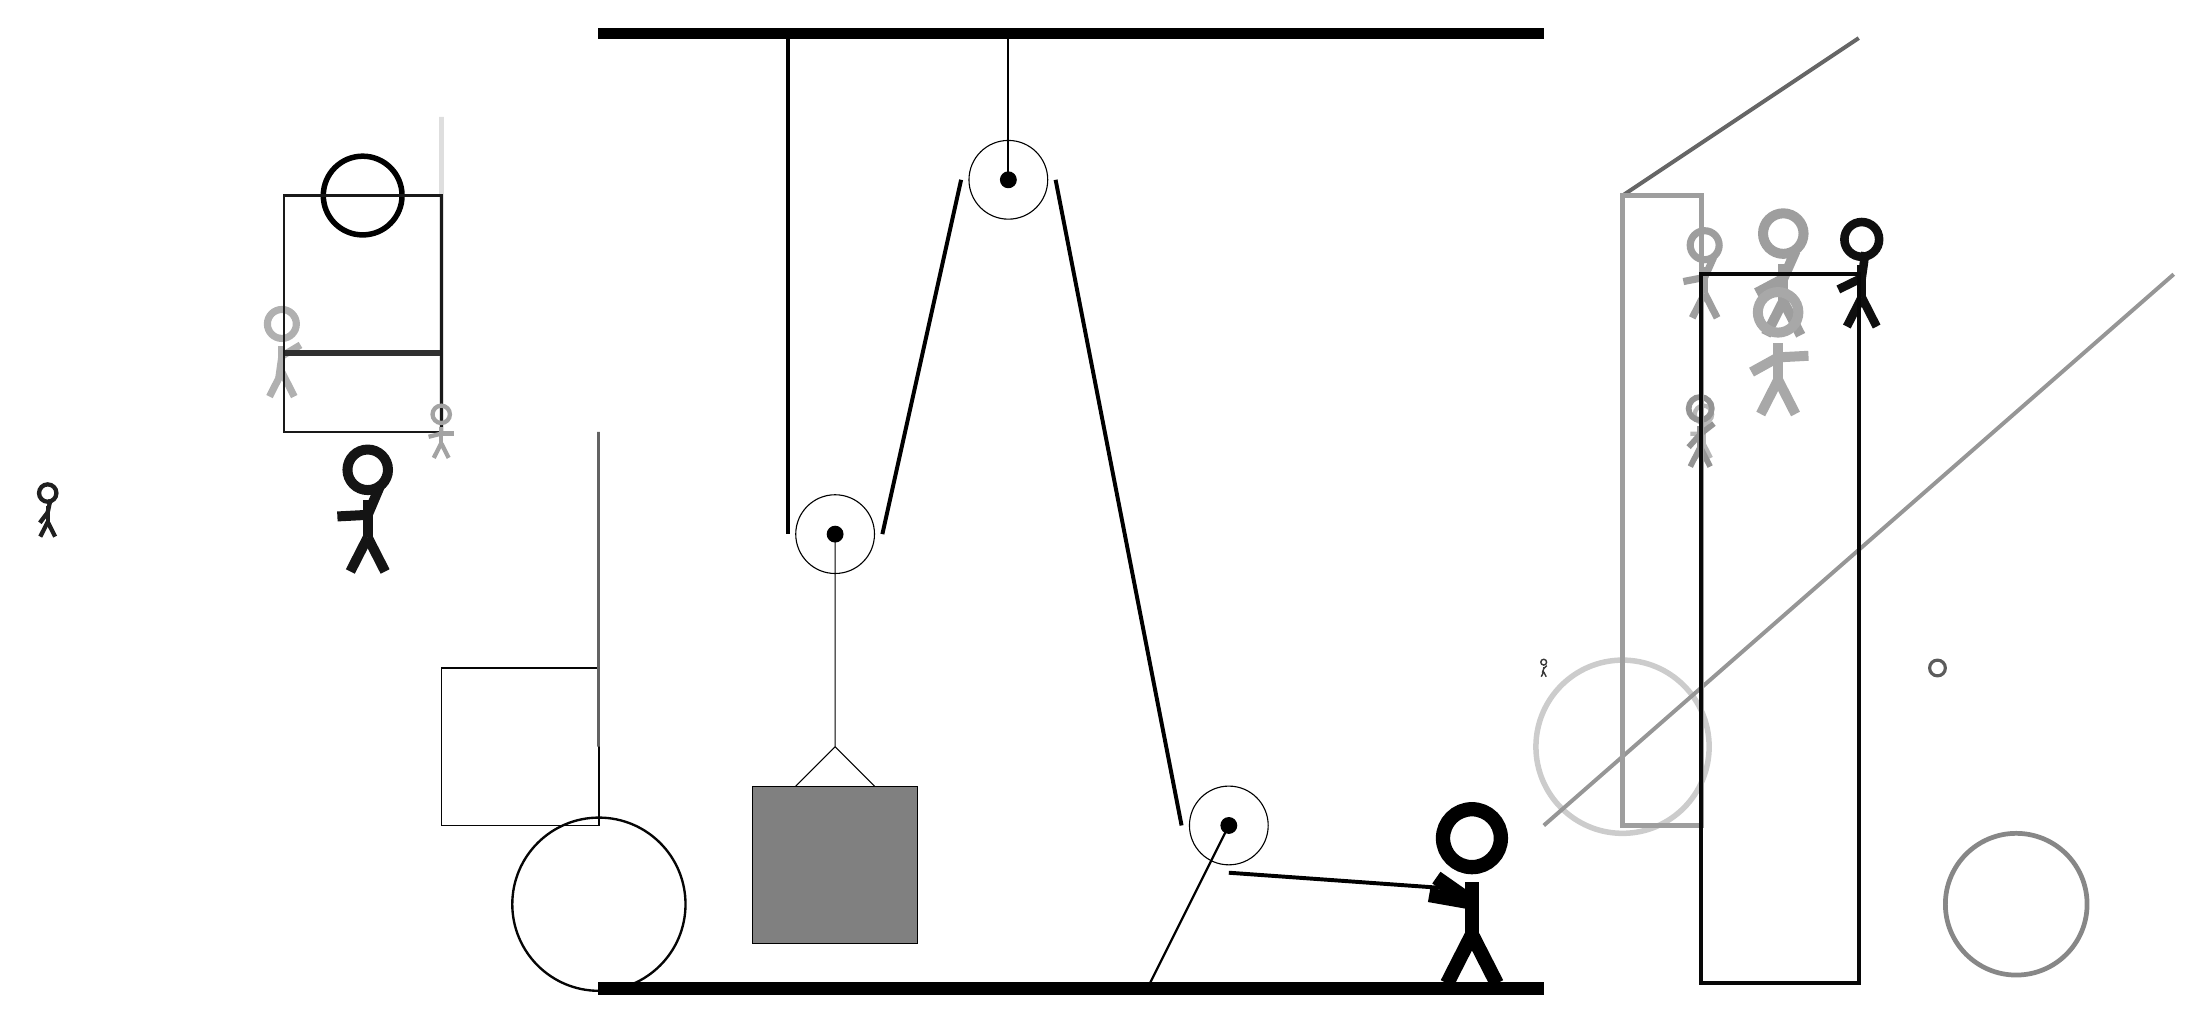
\begin{tikzpicture}
			%%%%% START %%%%%
			
			\draw[fill=black] (-2, 9) rectangle (10, 9.125);
			
			\draw (3.2, 7.2) circle (0.5);
			\draw[fill=black] (3.2, 7.2) circle (0.1);
			\draw[thick] (3.2, 7.2) -- (3.2, 9);
			
			\draw (6, -1) circle (0.5);
			\draw[fill=black] (6, -1) circle (0.1);
			\draw[thick] (6, -1) -- (5, -3);
			
			\draw (1, 2.7) circle (0.5);
			\draw[fill=black] (1, 2.7) circle (0.1);
			
			\draw (1, 2.7) -- (1, 0) -- (0.5, -0.5);
			\draw (1, 0) -- (1.5, -0.5);
			\draw[fill=black!50] (-0.05, -0.5) rectangle (2.05, -2.5);
			
			\draw[line width=0.5mm] (0.4, 9) -- (0.4, 2.7);
			\centerarc[line width=0.5mm](1, 2.7)(180:360:0.6);
			\draw[line width=0.5mm](1.6, 2.7) -- (2.6, 7.2);
			\centerarc[line width=0.5mm](3.2, 7.2)(0:180:0.6);
			\draw[line width=0.5mm](3.8, 7.2) -- (5.4, -1);
			\centerarc[line width=0.5mm](6, -1)(180:270:0.6);
			\draw[line width=0.5mm](6, -1.6) -- (8.8, -1.8);
			
			\draw[line width=0.5mm, color=black!60](14, 9) -- (11, 7);
			
			\draw[line width=0.2mm, color=black!98] (-2, -1) rectangle (-4, 1);
			\node[line width=0.6mm, color=black!28] at (12, 4) {\Strichmaxerl[3][1][74]};
			\node[line width=0.3mm, color=black!31] at (-6, 5) {\Strichmaxerl[5][82][31]};
			\draw [line width=0.7mm, color=black!100](-5, 7) circle (0.5);
			
			\draw[line width=0.6mm, color=black!13] (-4, 4) rectangle (-4, 8);
			\draw[line width=0.4mm, color=black!61] (-2, 4) rectangle (-2, 0);
			\node[line width=0.6mm, color=black!94] at (14, 6) {\Strichmaxerl[6][26][82]};
			\node[line width=0.4mm, color=black!88] at (-9, 3) {\Strichmaxerl[3][53][78]};
			\node[line width=0.5mm, color=black!42] at (12, 4) {\Strichmaxerl[4][48][38]};
			\draw [line width=0.3mm, color=black!98](-2, -2) circle (1.1);
			\draw [line width=0.7mm, color=black!20](11, 0) circle (1.1);
			\draw[line width=0.7mm, color=black!81] (-4, 5) rectangle (-6, 5);
			\node[line width=0.5mm, color=black!38] at (12, 6) {\Strichmaxerl[5][11][66]};
			\draw [line width=0.6mm, color=black!47](16, -2) circle (0.9);
			\node[line width=0.4mm, color=black!38] at (13, 6) {\Strichmaxerl[7][28][66]};
			
			\draw[line width=0.5mm, color=black!41](10, -1) -- (18, 6);
			\draw[line width=0.3mm, color=black!90] (-4, 7) rectangle (-6, 4);
			\node[line width=0.2mm, color=black!78] at (10, 1) {\Strichmaxerl[1][73][45]};
			\draw[line width=0.7mm, color=black!38] (12, -1) rectangle (11, 7);
			\draw [line width=0.4mm, color=black!64](15, 1) circle (0.1);
			
			\node[line width=0.3mm, color=black!92] at (-5, 3) {\Strichmaxerl[7][3][67]};
			\draw[line width=0.5mm, color=black!97] (12, -3) rectangle (14, 6);
			\draw[line width=0.5mm, color=black!43](13, 1) -- (13, 1);
			\node[line width=0.3mm, color=black!34] at (13, 5) {\Strichmaxerl[7][29][3]};
			
			\node[line width=0.4mm, color=black!36] at (-4, 4) {\Strichmaxerl[3][14][0]};
			
			
			\node at (9, -1.9) {\Strichmaxerl[10][-35][170]};
			
			\draw[fill=black] (-2, -3) rectangle (10, -3.15);
			
			%%%%% END %%%%%
		\end{tikzpicture}
	\end{figure}	
\end{document}